% !TEX root = ../final-main.tex
\chapter{Conclusions}
\label{ch:conclusions}

\section{Summary of Key Outcomes}

The central outcome of this project was the fabrication of enhancement-mode
GaAs/AlGaAs HEMTs using a recessed-gate process. The final non-oxide devices
showed positive threshold voltages, demonstrating that selective removal of the
donor-containing material beneath the gate could shift the device from
normally-on to normally-off operation. This satisfies the main aim of the work:
to investigate whether gate recession could be used to realise
enhancement-mode behaviour in the available GaAs/AlGaAs heterostructure.

\vspace{1mm}

The result was reached through three fabrication iterations, each of which
identified a different practical limit of the process. Iteration 1 showed that
the recessed region must control the full source--drain current path, rather
than only a local trench beneath part of the gate. Iteration 2 corrected this
geometry and improved gate control, but also showed that the wet recess etch was
highly sensitive to process conditions and could easily exceed the intended
depth. Iteration 3 introduced a pilot etch calibration immediately before
device processing, giving sufficient depth control to produce working
enhancement-mode devices.

\vspace{1mm}

It was not possible, however, to fabricate the full planned matrix of recess
depths across the quadrants. In the earlier iterations, the devices did not
show the intended behaviour, so the process direction had to change from simply
varying recess depth to correcting the gate geometry, recess geometry, and etch
control. Accurate measurement of the final recess depth was also extremely
challenging because the target depths were only a few tens of nanometres and the
recessed regions were defined within small gate features. For this reason, the
final comparison is presented in terms of etch time for devices processed in
the same etchant conditions. This does not provide an absolute recess depth for
each device, but it does provide a controlled comparison of the effect of
removing more material from the gate region. SEM cross sections were attempted
on the functioning devices, but locating the recessed region was not reliable
because of the small feature size and the roughness introduced at the
cross-sectioned edge.

\vspace{5mm}

\begin{figure}[htbp]
  \centering
  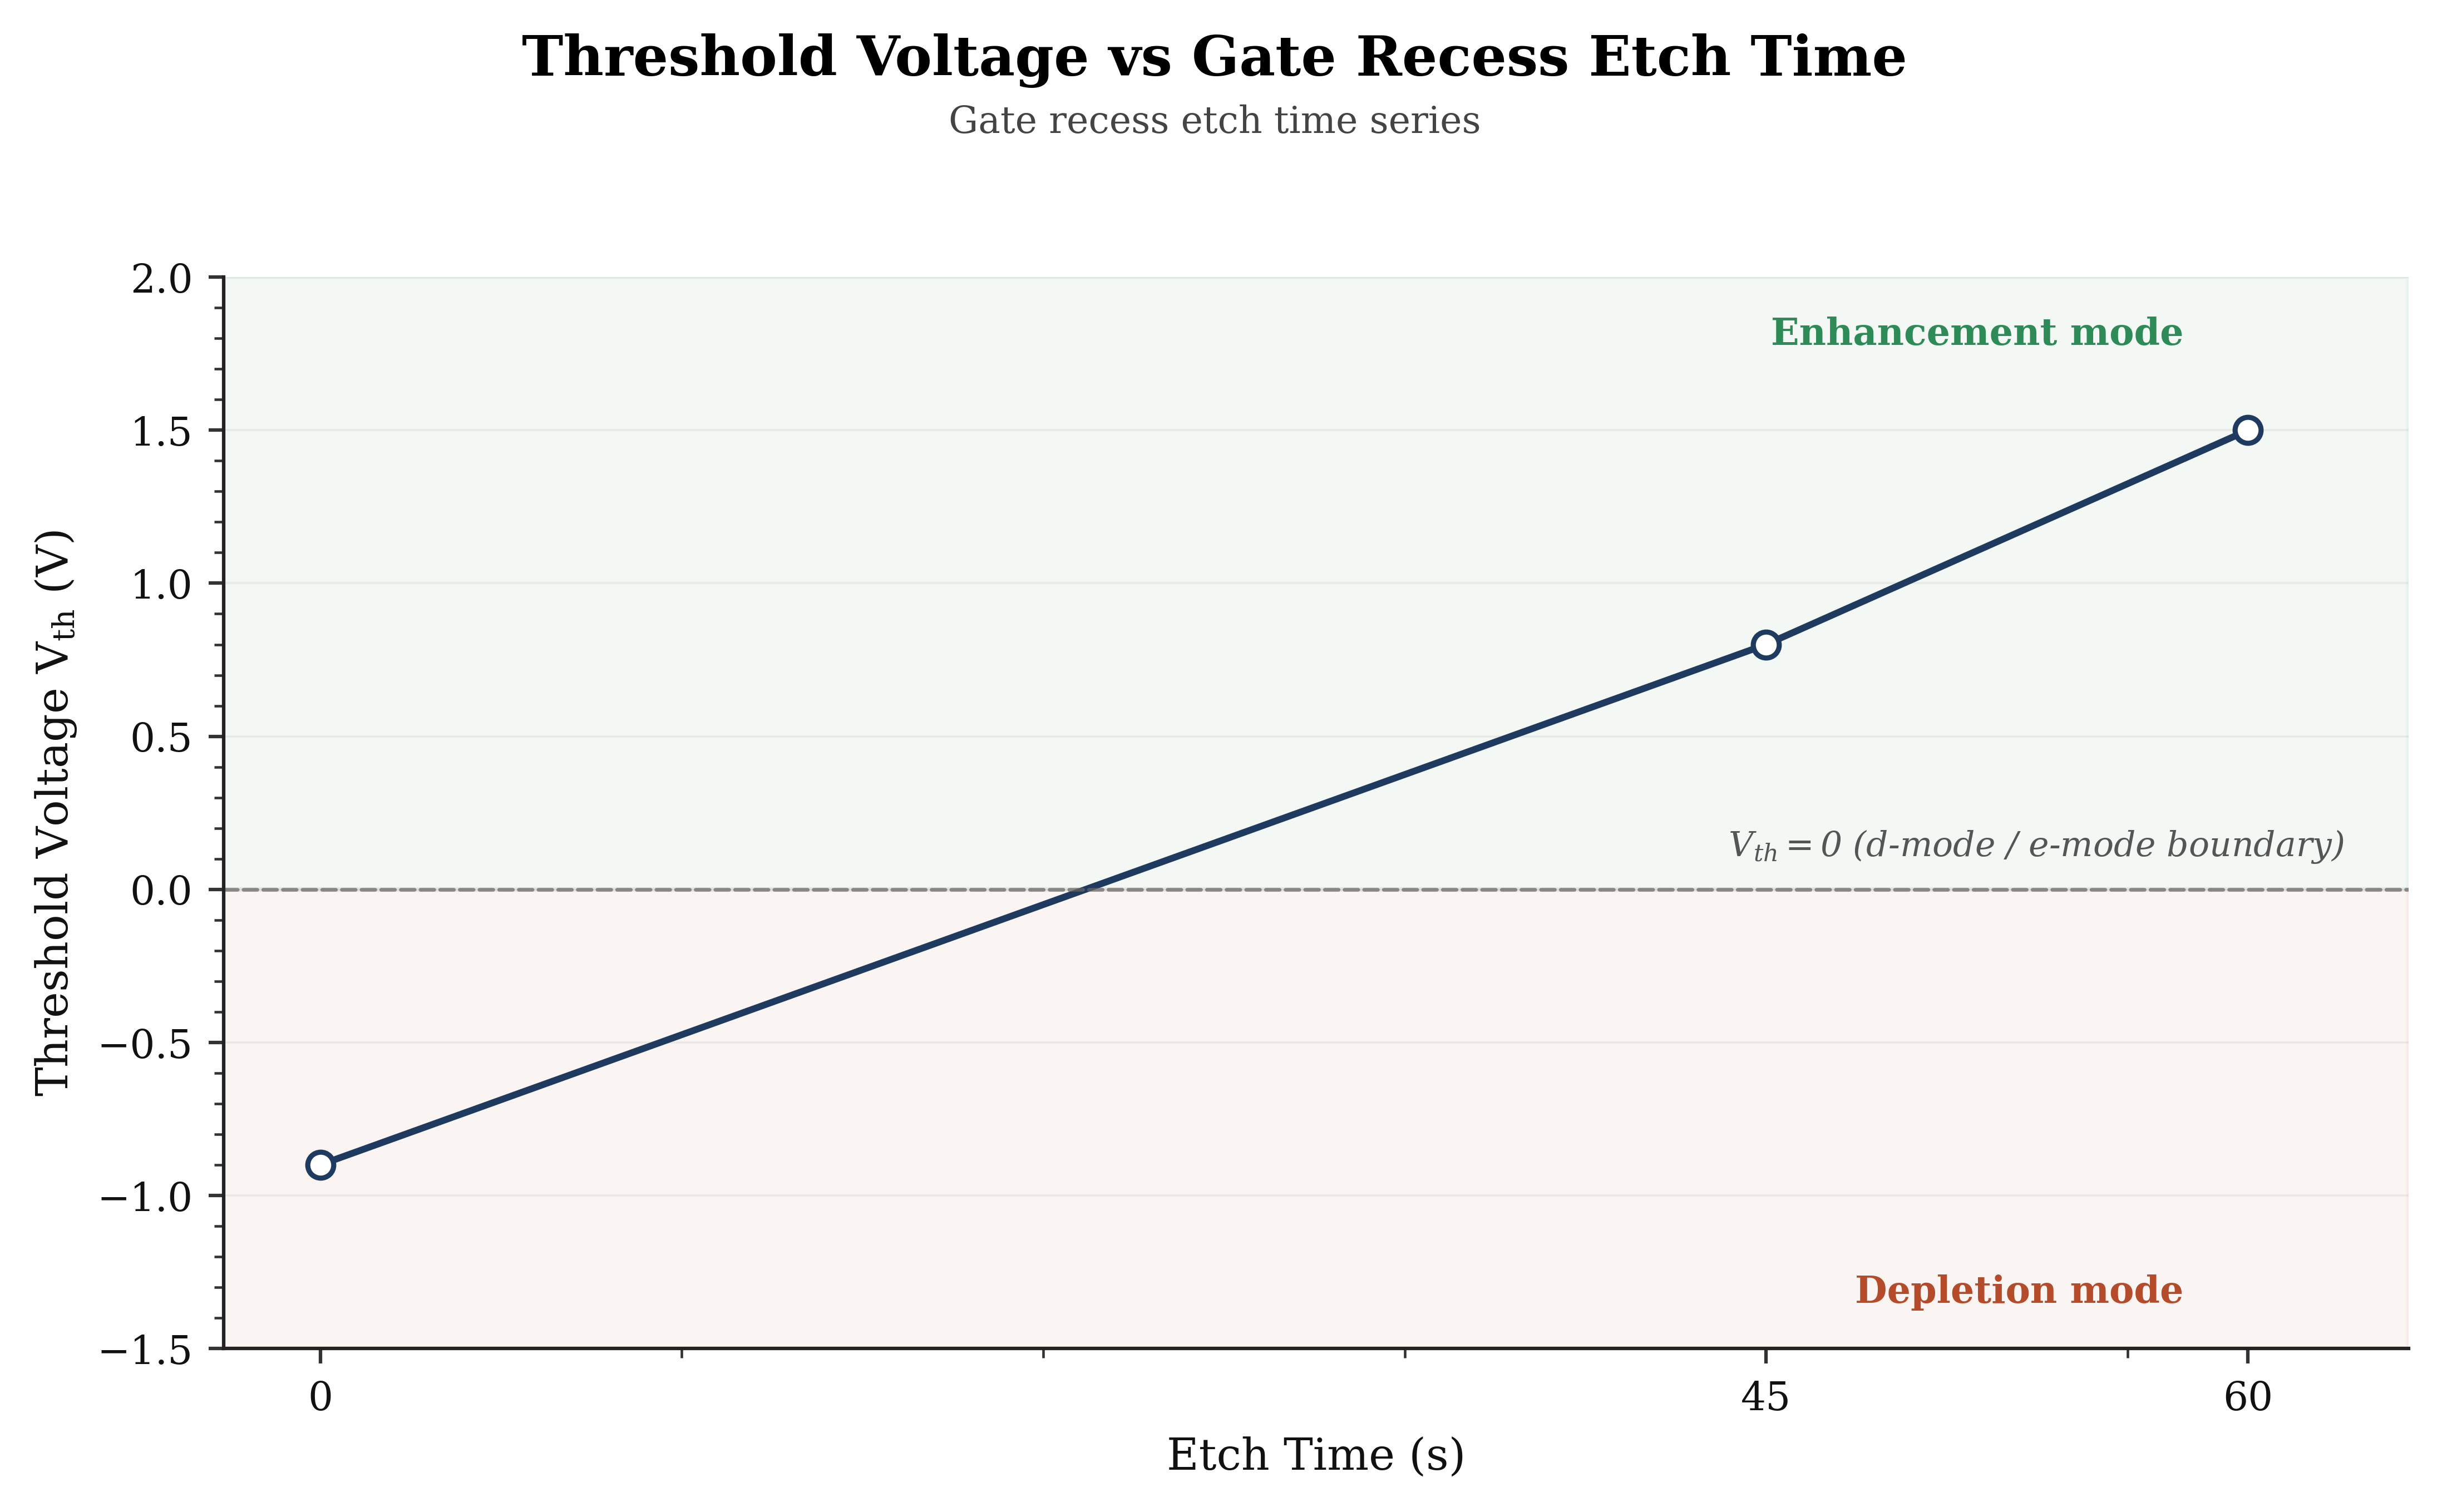
\includegraphics[width=1\linewidth]{figures/electrical_analysis/enhancement_mode/iteration_3/v_th_time.png}
  \caption{Threshold-voltage trend for the Iteration 3 recessed devices as a
  function of recess etch time.}
  \label{fig:v-th-time}
\end{figure}

Figure~\ref{fig:v-th-time} summarises the key electrical trend from the final
iteration. The device recessed for \SI{45}{\second} produced a threshold voltage
of approximately \SI{0.8}{\volt}, while the device recessed for
\SI{60}{\second} produced a threshold voltage of approximately
\SI{1.5}{\volt}. This supports the expected relationship between recess depth
and threshold voltage: a longer recess etch removes more donor material from
beneath the gate, reducing the zero-bias channel charge and requiring a more
positive gate voltage for conduction. The number of working final devices was
limited, so the data should not be treated as a full statistical process
calibration. Nevertheless, the measured trend is consistent with the physical
mechanism targeted by the project.

\section{Potential Applications}

The value of the devices fabricated in this project is not simply that a
positive threshold voltage was achieved, since normally-off behaviour can be
realised in other transistor technologies. The more specific contribution is the
demonstration of normally-off operation on a GaAs/AlGaAs HEMT platform. This
combines the circuit-level benefit of a positive threshold voltage with the
material advantages of a high-mobility III-V heterostructure. Such devices may
therefore be attractive in systems that already use GaAs HEMT technology, but
where depletion-mode operation introduces unwanted biasing complexity.

\vspace{1mm}

Relative to a depletion-mode HEMT, the key advantage is the zero-bias off state.
A depletion-mode device must be held off using a negative gate supply, whereas an
enhancement-mode device remains non-conducting until a positive gate voltage is
applied. This reduces the number of required bias rails and removes a potential
failure mode in which loss of the negative gate bias leaves the device
conducting. This behaviour is particularly useful in control applications, where
the preferred default state is off.

\vspace{1mm}

The most suitable applications are therefore likely to be low-current control
functions within GaAs-based circuits. Examples include RF front-end enable
switches, bias-selection networks, signal-routing switches, isolation switches
and protection paths. In these applications, the device is not required to
maximise current density; its value lies in providing a normally-off control
path that can be driven using a positive voltage while retaining the
high-frequency capability of III-V HEMT devices. A further use case is mixed
depletion/enhancement-mode GaAs logic, in which depletion-mode HEMTs provide
high-current or load functions while enhancement-mode HEMTs provide normally-off
switching.
